\chapter{WAV Designer}
WAV designer is a single-cycle waveform generator optimized for the Elektron MD.\\
It features a 3 oscillator additive synthesis engine with a level mixer.\\
\\
Each oscillator can be set to a unique waveform and pitch. The 3 oscillators are then mixed together and rendered in to a WAV file which can be transferred to the MD using the MIDI Sample Dump Specification (SDS).\\
\\
To ensure that the MD plays back the resulting waveform optimally, WAV Designer performs all the heavy lifting for you. This involves calculating sample length and rate based on the fundamental frequency, auto detecting loop points and normalizing the waveform.
\section{WAV Designer Pages}
\textit{WAV Designer is accessible from the \textbf{PageSelect} page and consists of 4 sub-pages. Once you have entered the WAV Designer you can access the sub-pages using the four Encoder buttons.}

\begin{itemize}
\item \textbf{Encoders[1-3]}: select Oscillator Pages 1-3 respectively.
\item \textbf{Encoder[4]}: is the Mixer Page.
\end{itemize}

\section{Oscillator Pages:}
\subsection{Encoder Assignment:}
\begin{itemize}
	\item \textbf{[ Encoder 1 ]: } Pitch, note increments.
	\item \textbf{[ Encoder 2 ]: } Fine Tune, +/- 100 cents
	\item \textbf{[ Encoder 3 ]: } Pulse Width
	\item \textbf{[ Encoder 4 ]: } Modify
\end{itemize}
\subsection{Pitch:}
Each oscillator can be tuned to a unique frequency.\\
\\The pitch is adjusted in note increments by rotating \textbf{[ Encoder 1 ]}. Rotating \textbf{[ Encoder 2 ]} will adjust the frequency in cents +/-100. Holding down \textbf{[ Shift 2 ]} will display the corresponding frequency.\\
\\The fundamental frequency of the rendered waveform is automatically selected from the oscillator that has the lowest frequency.
\subsection{Waveforms:}
Each oscillator can be set to a unique waveform by pressing the \textbf{[Save]} button from it's respective page.\\
\\
The available waveforms are described below:

\begin{itemize}
\item{\textbf{SIN:}}Sine waveform with adjustable overtones (each overtone is an octave above the fundamental frequency)\\
\fbox{
\includegraphics[scale=.40]{wav_designer_sine_init.png}}\\\\
\fbox{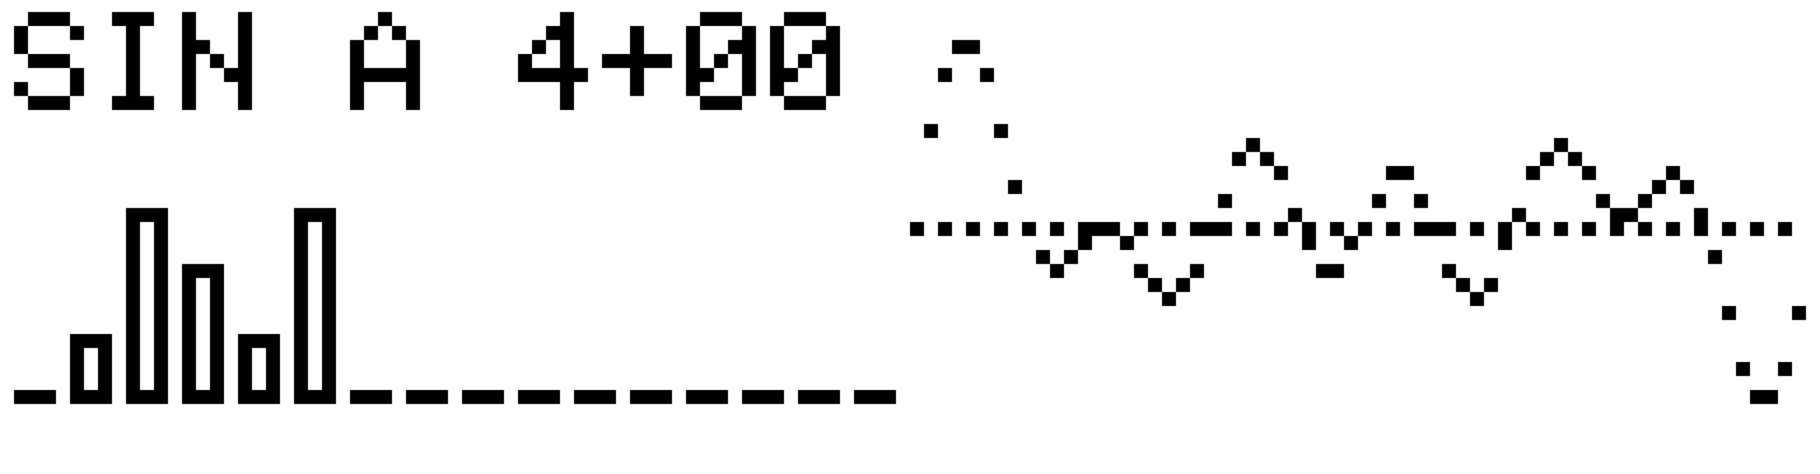
\includegraphics[scale=.40]{wav_designer_sin.png}}\\\\
\\Overtones are added by using the MD TI and rotating \textbf{[Encoder 4]}.
\item{\textbf{TRI:}} Triangle waveform with adjustable width.\\
\fbox{
\includegraphics[scale=.40]{wav_designer_tri.png}}\\\\
\item{\textbf{PUL:}} Pulse/Square waveform with adjustable width.\\
\fbox{
\includegraphics[scale=.40]{wav_designer_pulse.png}}\\\\
\item{\textbf{SAW:}}Sawthooth waveform with adjustable width\\
\fbox{
\includegraphics[scale=.40]{wav_designer_saw.png}}\\\\
\item{\textbf{USR:}}User defined waveform, 16 points with linear interpolation.\\
\fbox{
\includegraphics[scale=.40]{wav_designer_user.png}}\\\\
Sample values are modified by using the MD TI and rotating \textbf{[Encoder 4]}.
\end{itemize}
\subsection{Pulse Width:}
TRI, PULSE and SAW waveform's pulse width can be adjusted by rotating \textbf{[Encoder 3]}.\\
\fbox{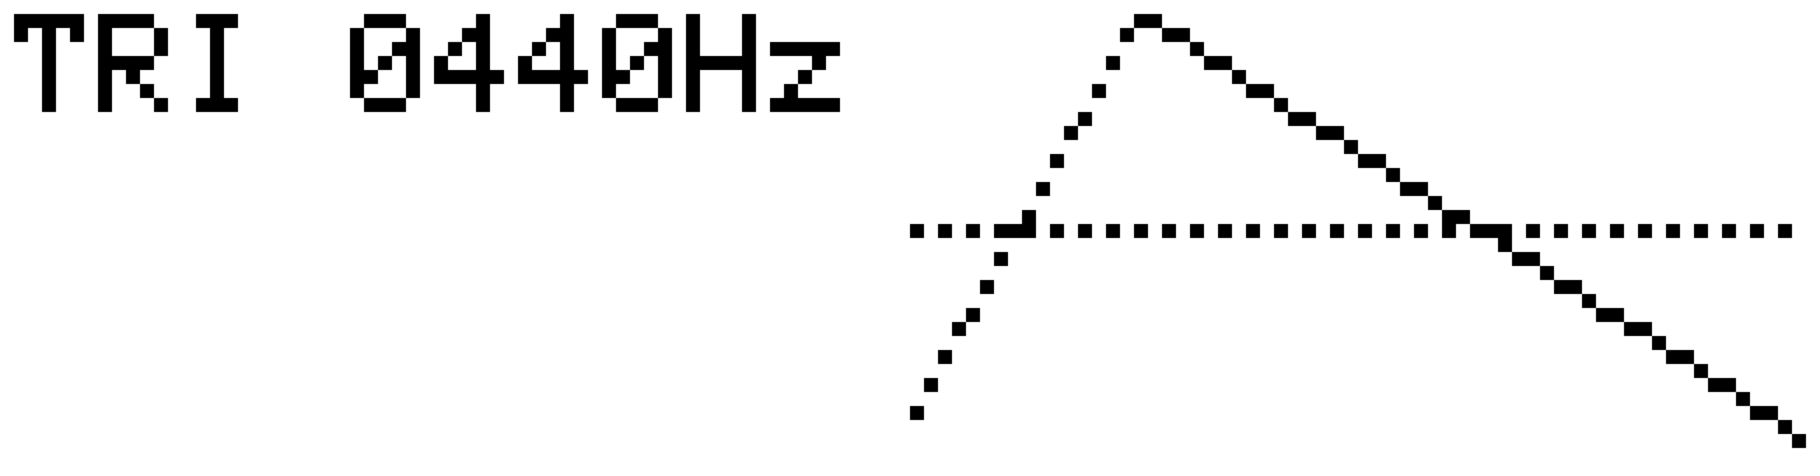
\includegraphics[scale=.40]{wav_designer_pulse_width.png}}\\
\newpage
\section{OSC Mixer Page:}
\fbox{
\includegraphics[scale=.40]{wav_designer_mixer.png}}\\\\
The Oscillator Mixer Page has volume levels for each of the oscillators which can be adjusted by rotating encoders 1 to 3. \textit{Absolute volume levels are not important here as the resulting waveform will be automatically normalized.}\\
\\The fourth encoder is used to set the sample slot position. On the MD the sample slots are offset by 1 (00 = 01).\\
\\
To render a sample and then transfer it to the MD's selected sample slot, press \textbf{[Write]}.\\
\\
For convience, pressing the \textbf{[Save]} button will open the SampleManager window on the MD. You can also choose the destination slot from here.
\subsubsection{Encoder Assignment:}
\begin{itemize}
	\item \textbf{[ Encoder 1 ]: } Osc1 Level
	\item \textbf{[ Encoder 2 ]: } Osc2 Level
	\item \textbf{[ Encoder 3 ]: } Osc3 Level
	\item \textbf{[ Encoder 4 ]: } Sample Slot
\end{itemize}
\textbf{Important}: The MD firmware features a nasty bug that causes the user interface to stop responding if a sample dump is received at any point after specific SYSEX messages are requested. As MCL uses SYSEX for all communication with the MD, the MD's GUI will lock up after a sample is received from WavDesigner. The only known work around at this time is to reset the MD.